\chapter{Design}



\subsection{Stakeholders}

\newcommand{\primary}{\hlc{cyan}{ PRIMARY }\\}
\newcommand{\secondary}{\hlc{yellow}{ SECONDARY }\\}
\newcommand{\tertiary}{\hlc{green}{ TERTIARY }\\}

\paragraph{Game Developers}\primary
This group will use the application to release their games and its updates to their users, who they will reward for helping to distribute it.

\paragraph{Players}\primary
This group will use this application to downloaded and update their games off of. They may also contribute to the distribution of the games to other players for an incentive provided by the developers.

\paragraph{Game Distribution Platforms}\secondary
This group consists of platforms like Steam or Epic Games, which serve as the main competitor to this application. It is likely that as more developers choose this application, this group will see a loss in revenue. 

\paragraph{}\tertiary

\section{Stakeholders \& Requirements}


\subsection{Stakeholders}

\newcommand{\primary}{\hlc{cyan}{ PRIMARY }\\}
\newcommand{\secondary}{\hlc{yellow}{ SECONDARY }\\}
\newcommand{\tertiary}{\hlc{green}{ TERTIARY }\\}

\paragraph{Game Developers}\primary
This group will use the application to release their games and its updates to their users, who they will reward for helping to distribute it.

\paragraph{Players}\primary
This group will use this application to downloaded and update their games off of. They may also contribute to the distribution of the games to other players for an incentive provided by the developers.

\paragraph{Game Distribution Platforms}\secondary
This group consists of platforms like Steam or Epic Games, which serve as the main competitor to this application. It is likely that as more developers choose this application, this group will see a loss in revenue. 

\paragraph{}\tertiary

\subsection{Requirements}

Tables~\ref{tab:functional-requirements} and~\ref{tab:non-functional-requirements} show the functional and non-functional requirements of this project organized using MoSCoW prioritisation. 

\subsubsection*{Functional Requirements}

\begin{longtable}{ p{.1\textwidth} p{.8\textwidth} }
  \toprule
  \textbf{ID} & \textbf{Description}
  \\\midrule\midrule
  \multicolumn{2}{c}{\cellcolor{red!70}\textit{Must}}\\\midrule
  F\_M1 & Store software metadata on a blockchain\\
  F\_M2 & A node must request individual shards from its peers\\
  F\_M3 & A node must be able to discover peers relevant to the software it wants\\
  F\_M4 & Software must be updatable through the blockchain\\
  F\_M5 & A node must be able to upload software\\
  F\_M6 & A node must be able to download software in its entirety from nodes in the same network.\\
  F\_M7 & A node must be able to verify the integrity of each block it downloads\\
  F\_M8 & The application should run on the Ethereum network\\
  F\_M9 & Users must be able to purchase games from developers over the network\\
  F\_M10 & Users must be able to prove they have purchased a game\\
  \midrule\multicolumn{2}{c}{\cellcolor{orange!70}\textit{Should}}\\\midrule
  F\_S1 & Seeders should have a way to prove how much data they have seeded\\
  F\_S2 & Seeders will only upload content to users who have a valid proof of purchase\\
  \midrule\multicolumn{2}{c}{\cellcolor{green}\textit{Could}}\\\midrule
  F\_C1 & Allow users to request specific software versions\\
  \midrule
  \bottomrule
  \label{tab:functional-requirements}
\end{longtable}

\subsubsection*{Non-Functional Requirements}

\begin{longtable}{ p{.1\textwidth} p{.8\textwidth} }
  \toprule
  \textbf{ID} & \textbf{Description}
  \\\midrule\midrule
  \multicolumn{2}{c}{\cellcolor{red!70}\textit{Must}}\\\midrule
  NF\_M1 & The application is decentralized and cannot be controlled by any one party\\
  NF\_M2 & Any user must be able to join and contribute to the network\\
  NF\_M3 & Game uploaders should be publicly identifiable\\
  NF\_M4 & Metadata required to download the game should be immutable\\
  \midrule\multicolumn{2}{c}{\cellcolor{orange!70}\textit{Should}}\\\midrule
  NF\_S1 & This application must be scalable, such that many users can upload and download the same game at the same time.\\
  NF\_S2 & Only the original uploader can upload an update to their game\\
  \midrule\multicolumn{2}{c}{\cellcolor{green}\textit{Could}}\\\midrule
  \\
  \midrule
  \bottomrule
  \label{tab:non-functional-requirements}
\end{longtable}

\section{Design Considerations}

This section will give a high-level design showing how each of the functional requirements can be met by considering key functions for the applications.

% chktex-file 24
% chktex-file 8

\subsection{Data}
\label{subsec:design-data}

Table~\ref{tab:data} discusses the different types of data we are going to need to store and where they should be stored based upon their properties.


\begin{longtable}{ p{.12\textwidth} p{.1\textwidth} p{.1\textwidth} p{.63\textwidth} }
  \toprule
  \textbf{Data} & \textbf{Size} & \textbf{Location} & \textbf{Explanation}\\
  \midrule\midrule
  Game Metadata\newline\reqref{F-M1}
  & 100 -- \newline200B
  & Ethereum
  & This data is the minimal set of information required for the unique identification of each game. See Section~\ref{subsubsec:eth-data}.

  \vspace{1mm}
  This data is appropriate to store on Ethereum as it is public, small in size, and essential to the correct functioning of the application as all users will need to be able to discover all games. 
  \x
  Game Hash Tree\newline\reqref{F-M12}
  & \~15KB
  & IPFS
  & This will be the compressed Hash Tree that will allow the users to identify and verify the shards of data they need to download for their game. The user will download this immediately after purchasing the game.

  \vspace{1mm}
  This data would be costly to store on Ethereum for a large number of games and will only need to be accessed by a subset of users. As it is also public data, IPFS is appropriate to store it on, and we can reference the CID within the data stored on Ethereum.
  \x
  Game\newline Assets\newline\reqref{F-C2}
  & Unkown~\footnote{Some games may include many promotional materials, whilst some could include none. Therefore, it is hard to estimate the expected size.} 
  & IPFS
  & This will represent any promotional material provided for the game that can be viewed on the game's store page. This will typically include cover art and a markdown file for the description. The user will download this when they first view it in the store.

  \vspace{1mm}
  Similar to the Hash Tree, this will typically be too large to store on Ethereum so, given that it is public and non-essential data, IPFS will be used to store and distribute it. 
  \x
  Game Data
  & \textit{avg. 44GB~\footnote{Calculated based off of the top 30 games from SteamDB~\cite{noauthor_steam_nodate}.}}
  & Peers
  & This will the data required to play the game and will be fetched based upon the contents of the game's Hash Tree.

  \vspace{1mm}
  This data is way too large to store on Ethereum but also isn't public, which means using IPFS would not be appropriate~\footnote{IPFS and similar platforms provide no access control for the data stored there and any encryption based technique would be unviable.}. Therefore, this project will use a custom P2P network for sharing data, which is described in Section~\ref{subsec:design-p2p} 
  \\\bottomrule\bottomrule
  \caption{The different types of data required for each game.}
  \label{tab:data}
\end{longtable}

\noindent 
Swarm~\cite{hartman_swarm_1999} was considered as a decentralised storage and distribution platform over IPFS but was decided against as it would couple this project more tightly with Ethereum. On top of that, IPFS has much greater adoption and is much more mature in terms of working on a large scale.

\subsection*{Blockchain}\label{subsec:design-con-eth}

\subsubsection*{Type of Blockchain}

To satisfy \reqref{NF-M1} and \reqref{NF-M2}, we will need to use a public blockchain. This will benefit my project by:
\vspace{2mm}
\begin{itemize}
  \item being accessible to more users, which will boost both availability and scalability \reqref{NF-S1},
  \item reducing the risk of censorship \reqref{NF-M1}, and
  \item providing greater data integrity \reqref{NF-M4}
\end{itemize}

\newparagraph Ethereum is a public blockchain that allows developers to publish their own distributed applications to it. It comes with an extensive development toolchain so is an obvious choice for this project \reqref{F-M4}.

\subsubsection*{Uploading Games}
\label{subsubsec:eth-data}



To satisfy \reqref{F-M1} and \reqref{F-M2}, the data stored on the blockchain will be used for the identification of games. Table~\ref{tab:eth-data} shows the fields that will stored as part of the smart contract for each game and to manage the whole collection of games. Fields in \textit{italics} are generated for the user and non-italic fields are entered manually.

\begin{longtable}{ p{.2\textwidth} p{.75\textwidth} }
  \toprule
  \textbf{Name} & \textbf{Description}
  \\\midrule\midrule
  \multicolumn{2}{c}{\textit{Metadata for each game}} 
  \\\midrule\midrule
  title & The name of the game.\\
  version & The version number of the game.\\
  \textit{release date} & The timestamp for when the game was uploaded.\\
  developer & The name of the developer uploading the game \reqref{NF-M3}.\\
  \textit{uploader} & The Ethereum address of the developer \reqref{NF-M3}.\\
  \textit{root hash} & The root hash of the game that uniquely identifies the game and is based upon its contents.\\
  previous version & The root hash of the most previous version of the game if it exists.\\
  price & The price of the game in Wei.\\
  \textit{hash tree CID} & Required for downloading the hash tree from IPFS.\\
  \textit{assets CID} & Required for downloading the assets folder from IPFS.
  \\\midrule\midrule
  \multicolumn{2}{c}{\textit{Managing the Collection of Games}} 
  \\\midrule\midrule
  \textit{library} & A mapping for all games uploaded to the network, where a game's root hash is the key used to find its metadata.\\
  \textit{game hashes} & Solidity doesn't allow us to enumerate maps so we will also store a list of hashes for all games uploaded.\\
  \textit{purchased} & A mapping which allows us to easily check if a user has purchased a game \reqref{F-M6}.
  \\\bottomrule\bottomrule
  \caption{the data to be stored on Ethereum using a smart contract}
  \label{tab:eth-data}
\end{longtable}


\subsubsection*{Purchasing Content}

Users will purchase games from developers over Ethereum by transferring Ether \reqref{F-M5}. The user's address will then be added to a public record, on the smart contract, of all users who have purchased the game \reqref{F-M6}. Upon purchasing a game, a user will broadcast their new library to all of their peers.

% chktex-file 1
% chktex-file 13

\subsection{Distributed File Sharing}
\label{subsec:design-p2p}

\subsubsection*{Hash Tree}
\label{subsubsec:hash-tree}

The hash tree of a given directory is used to represent its structure as well as the contents of its files. Each file is represented by an ordered list of SHA-256 hashes that match a fixed-size block of data. This allows users to easily identify and verify game data \reqref{F-M10}.

\begin{figure}[ht]
  \centering
  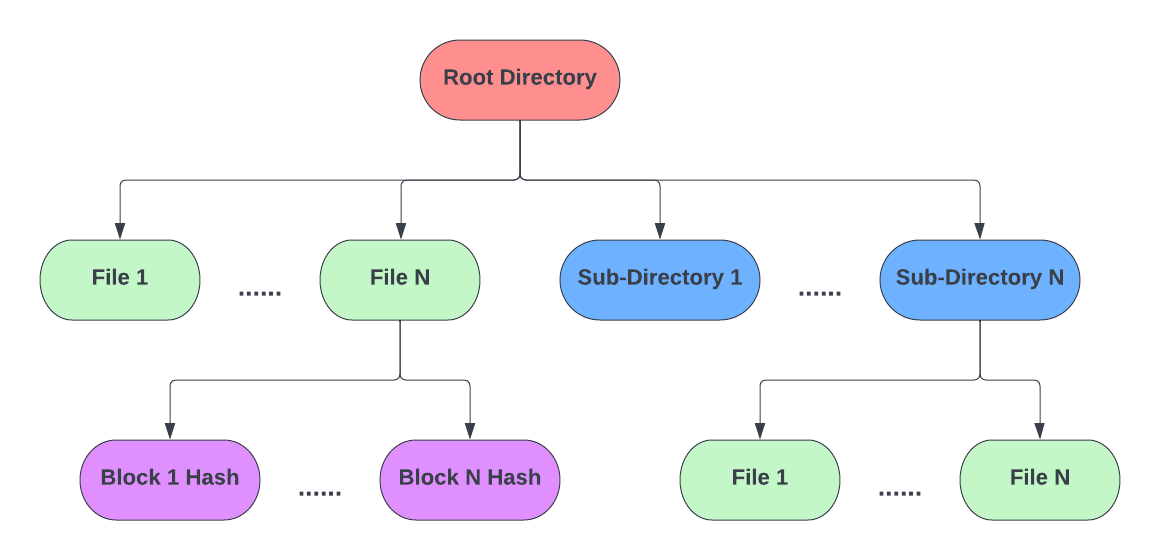
\includegraphics[width=.85\textwidth]{assets/images/diagrams/block-body.png}
  \caption{The structure of a hash tree}
  \label{fig:hash-storage}
\end{figure}

\subsubsection*{Uploading Content}
\label{subsubsec:upload-content}

For a developer to upload their game \reqref{F-M1}, they must provide the following:

\begin{itemize}
  \item the metadata outlined in Section~\ref{subsubsec:eth-data},
  \item a hash tree created from the root directory of the game, and
  \item an assets folder containing a piece of cover art \textit{(cover.png)} and a description file \textit{(description.md)}.
\end{itemize}

\vspace{2mm}\noindent
The developer should be able to enter the required fields into an upload page of the GUI and have the data generated and uploaded for them \reqref{F-S2}.

\subsubsection*{Downloading Content}

\newcommand{\seeder}{$P_{seeder}$~}
\newcommand{\downloader}{$P_{downloader}$~}

Like mentioned in Section~\ref{subsec:design-data}, it is impractical to store the game's data on the blockchain or IPFS. Instead we will consider ideas from decentralised file-sharing networks, like discussed in Sections~\ref{sec:lit-p2p} \&~\ref{sec:bittorrent}.
\x
Games are content addressable using their root hash field, which will allow users to request data from that game from other users. When a peer seeking data \downloader forms a connection with another peer \seeder they will:

\begin{enumerate}
  \item Perform a handshake to determine each other's Ethereum address and public key.
  \item \seeder will verify that \downloader owns the game by checking the \textit{purchased} mapping on the smart contract \reqref{F-M6} \reqref{F-S1}.
  \item \downloader will send requests for individual blocks to \seeder \reqref{F-M9}.
  \item Upon receiving a block, \downloader will verify the contents using the block's hash \reqref{F-M10} before writing it to disk in the appropriate location.
  \item Repeat Steps 3--4 until the entire game has been downloaded \reqref{F-M11}.
  \item \seeder may request a signed receipt that details the blocks they uploaded \reqref{F-S3} to \downloader.
\end{enumerate}

\vspace{2mm}\noindent
Users will be able to connect to many peers at once \reqref{F-M7} and will send download requests to the subset of their peers who also own the game. Requests will be sent in a round-robin fashion to evenly distribute the requests and prevent overloading a single peer \reqref{NF-S1}. Requests that cannot be completed will be retried when connecting to a new peer or when a peer has a change in library.

\subsubsection*{Updating Content}\label{subsubsec:updating}

To satisfy \reqref{F-M2}, developers will perform the same steps outlined in Section~\ref{subsubsec:upload-content} but must also provide the root hash of the most previous version of the game. Any users who have purchased the previous version will be added to the list of users who have purchased the new version \reqref{F-M3}. Additionally, this will include the restriction that only the original uploader can upload an update for their game \reqref{NF-M5}.
\x
Each version is considered its own game and will require users to download the updated version separately. Whilst this isn't reflective of how updates are typically managed, this will be acceptable for the scope of this project.

\subsubsection*{Downloadable Content}

Downloadable Content (DLC) \reqref{F-C1} represent optional additions for games that users will buy separately. DLCs will act similarly to how updates are treated. Each DLC will need:

\begin{enumerate}
  \item \textbf{Dependency} The root hash of the oldest version of the game this DLC supports.
  \item \textbf{Previous Version} (Optional) The root hash of the previous version of the DLC.
\end{enumerate}

\vspace{2mm}\noindent
Users must own the original game to buy any of its DLC. 

\subsubsection*{Proving Contribution}

As a user downloads blocks of data, they will keep track of which users have sent them which blocks. A peer may then request their contributions in the form of a signed message that can be sent to the developer \reqref{F-S3} in return for some kind of reward. The contents of the reward isn't specified for this project but could include in-game items, digital assets or Ether. This solution assumes that developers have knowledge of which Ethereum address maps to which of their game's users.

\section{Architecture}

This application uses the Model-View-Controller MVC pattern to structure the application to create a separation of concern between the main layers of the application. Figure~\ref{fig:impl-layers} shows a high level overview of the architecture and below I discuss the purpose for each.

\begin{figure}[ht]
  \centering
  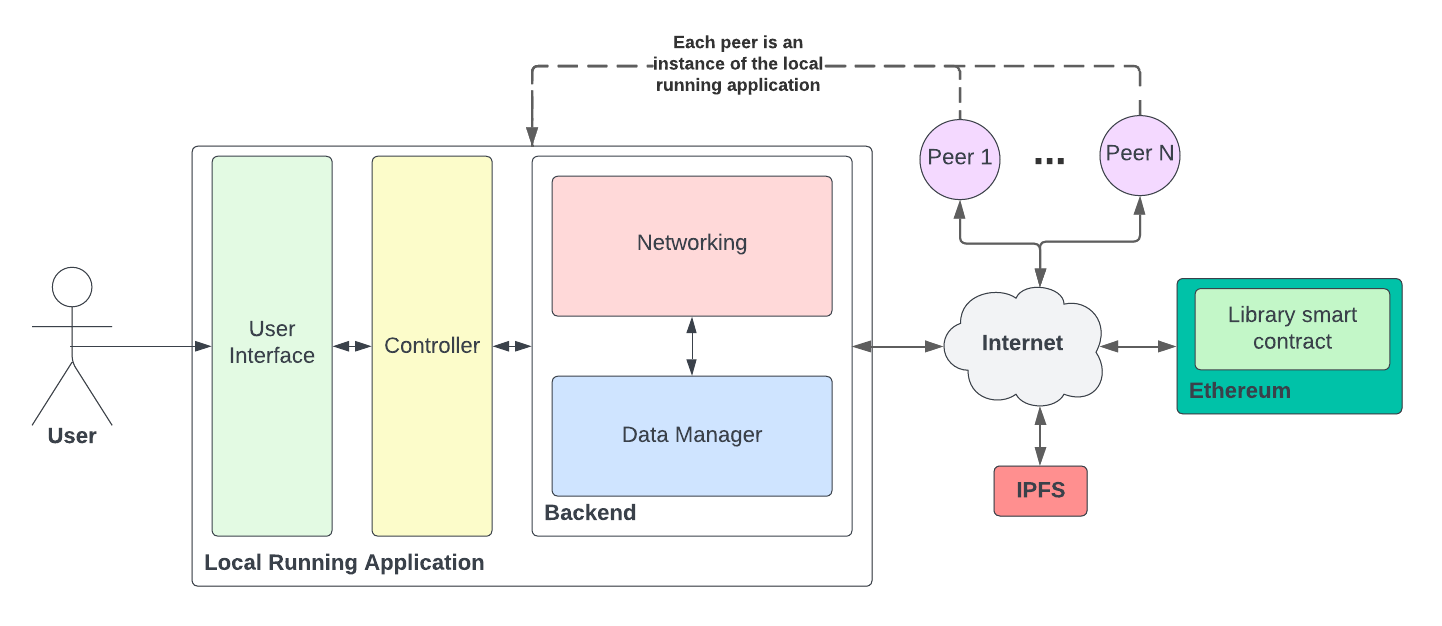
\includegraphics[width=.8\textwidth]{assets/images/diagrams/layers.png}
  \caption{The layers of the application}
  \label{fig:impl-layers}
\end{figure}

% layer entries


\subsection{Persistence}

The Persistence layer shows how the data for the application is divided across several mediums; namely the \textbf{Ethereum Smart Contract}, \textbf{IPFS}, and a \textbf{P2P Network}. Each component stores a different, which is outlined in Section~\ref{subsec:design-data}.
\x
There are several things to note about using Ethereum as platform for selling games:

\begin{itemize}
  \item Ethereum is a less stable currency than most traditional currencies like GBP or USD so games may fluctuate largely in price.
  \item All write functions on the smart contract will incur a gas fee so uploading or updating data will not be free.
  \item Users will have to source Ether from elsewhere before being able to purchase games, which may be intimidating to users not already familiar with the ecosystem.
\end{itemize}

% \subsubsection{Ethereum}\label{subsubsec:impl-eth}

% An Ethereum Smart Contract, written in Solidity \url{https://docs.soliditylang.org/en/v0.8.19/}, will be used to store the set of data about games that is required for the identification of each game. The Smart Contract will also be used to perform the following:
% \x
% The Geth go-ethereum package \url{https://geth.ethereum.org/} will allow us to interact with the ethereum blockchain and Abigen \url{https://docs.avax.network/specs/abigen} will allow us to compile any smart contracts to Go code. This will allow us to interact with our smart contract on ethereum using a set of Go functions. For development, Ganache \url{https://github.com/trufflesuite/ganache} was used to create a local Ethereum instance and Geth was used to connect to an Ethereum test net.


% \subsubsection{IPFS}

% This project will use the IPFS implementation Kubo \url{https://github.com/ipfs/kubo}, due to it being the most widely used implementation of IPFS. We will use the go-ipfs-api library \url{https://github.com/ipfs/go-ipfs-api} to interact with Kubo and upload/download the data specified above.


\subsection*{Backend}\label{subsec:backend}

The Backend can be broken down into two major components:

\begin{itemize}
  \item \textbf{Networking} The creation and maintenance of network connections with other peers over the internet with the purpose of sharing data.
  \item \textbf{Data Manager} the management of local data and the processing of data received and to be uploaded by the Networking component.
\end{itemize}

\subsubsection{Networking}\label{subsubsec:networking}

This component will connect users to the distributed P2P file-sharing network, where it will create and maintain a set of TCP connections with other users \reqref{F-M7} in the network and will communicate by sending structured messages to each other \reqref{F-M8}. Section~\ref{subsubsec:commands} describes these commands in detail.

\paragraph*{Peer Identification}
Peers are identified by their Ethereum addresses, which will allow us to view which games they've purchased and are allowed access to. Upon forming a connection, each peer will request the other return a signature for a generated message, from which we can derive their address and public key.

\paragraph*{Commands}\label{subsubsec:commands}

Structured messages \reqref{F-M8} will typically come as part of a request/response pair involving the sharing of information between peers. Command responses are not awaited to remove unnecessary blocking of the connection channel as a user may be responding to many different requests at once by the same peer. Table~\ref{tab:network-cmds} shows the list of commands used bu the application.

\small
\begin{longtable}{p{.38\textwidth} p{.57\textwidth}}
  \toprule
  \textbf{Message Format} & \textbf{Description}\\
  \midrule\midrule
  LIBRARY
  & Request that a peer sends their library of game.\\
  GAMES;$[hash_1]$;$[hash_2]$;\ldots;
  & The user sends a list of their games as a series of unique root hashes. These root hashes will map to games on the blockchain.\\
  \midrule
  BLOCK;$[gameHash]$;$[blockHash]$;
  & The user will request a block of data off of a peer by sending the root hash of the game and the hash of the block being requested. The response will be a SEND\_BLOCK message \reqref{F-M9} and if it isn't received after a given amount of time then it is resent.\\
  SEND\_BLOCK;$[gameHash]$;\newline $[blockHash]$;$[compressedData]$;
  & The user sends a block of data in response to a BLOCK message \reqref{F-M9}. The data is compressed using the \textit{compress/flate} package to reduce message size \reqref{NF-S1}.\\
  \midrule
  VALIDATE\_REQ;$[message]$
  & The user is requesting for a message to be signed using the receiver's Ethereum private key. This is used to verify the receiver's identity and thus their owned collection of games \reqref{F-S1}.\\
  VALIDATE\_RES;$[signed message]$
  & The user responds to a VALIDATE\_REQ message with a signed version of the received message. From this signature, the receiver can determine the address and public key of the user \reqref{F-S1}.\\
  \midrule
  REQ\_RECEIPT;$[gameHash]$
  & A user will request a RECEIPT message from a peer detailing the data that has been sent by the user for a specific game \reqref{F-S3}.\\
  RECEIPT;$[gameHash]$;$[signature]$\newline ;$[message]$
  & A user will respond to a REQ\_RECEIPT message with a signed message detailing all of the blocks that the requester has sent to the user from a given game. This will allow for users to prove their contributions to the game developer who could then reward them \reqref{F-S3}.\\
  \midrule
  REQ\_PEERS
  & A user requests the list of peers which the receiver peer is connected to. This will be sent immediately after a peer's identity is validated and will help increase the connectivity in the network \reqref{F-S4}.\\
  PEERS;$[p_1 hostname]:[p_1 port]$;\ldots
  & A user will send a list of their active peers. This will be limited to those peers which they have connected to and thus know the hostname and port of their server \reqref{F-S4}.\\
  SERVER;$[hostname]:[port]$
  & When we form a connection with a peer we send them the address of our server that peers use to connect to us. This allows that peer to share our address through the PEER command so we are more easily discoverable.\\
  \midrule
  ERROR;$[message]$
  & An error message that can be used to prompt a peer to resend a message.\\
  \bottomrule\bottomrule
  \caption{The set of structured messages sent between peers}
  \label{tab:network-cmds}
\end{longtable}
\normalsize
\subsubsection{Data Manager}\label{subsubsec:data-manager}

This component is responsible for interacting with local storage and managing the user's collection of owned and installed games.
It will interact directly with Ethereum to discover, purchase \reqref{F-M5}, and upload \reqref{F-M1} \reqref{F-M2} games and use IPFS to upload and distribute game assets \reqref{F-C2} and hash trees \reqref{F-M12}.

\paragraph*{Download Order} Each download will have a downloader thread that selects the order at which blocks are to be fetched. Using the hash tree, it will queue whole files at a time and to verify the whole file once all blocks have been fetched.





\subsubsection*{Optimisations}

\paragraph*{Worker Pools}
Tasks are queued down a FIFO channel and each one is collected by a single worker thread who will perform a specific task based upon what data was sent. This allowed us to have many worker threads listening on the same channel who will complete tasks in parallel to largely increase the performance of the application.

\vspace{2mm}\noindent
Some of the areas this pattern was used include:

\begin{itemize}
  \item Sharding files to create a hash tree,
  \item To locate and request blocks from many downloads at once, and
  \item To insert received data and free up the thread listening on a connection,
\end{itemize}

\paragraph*{Ignore File} A standard implementation of a .ignore file was included to indicate to the hash tree algorithm which files/folders to ignore. This is useful to ignore temporary or non-static files, which contents will vary by user and thus won't need to be distributed.

\subsection*{Frontend \& Controller}

\subsubsection{Frontend}\label{subsubsec:frontend}

This application will have a GUI \reqref{F-S2} \reqref{NF-S2} where users can interact with the platform. Having a GUI is essential to making the platform as easy to use as possible so that it is accessible to new users. At minimum it will need to include the following pages:

\begin{itemize}
  \item \textbf{Library} The user's collection of owned games, where they can view details for each game as well as manage their download status.
  \item \textbf{Store} Where user's can find and purchase new games that have been uploaded by other users.
  \item \textbf{Upload} Where users can fill in details about their new or updated game and have it be uploaded to the network.
  \item \textbf{Downloads} Where user's can track all of their ongoing downloads and see their progress.
  \item \textbf{Peers} Where users can manage their list of connected peers. Here a user can form new connections, break existing ones and request specific data from their peers.
  \item \textbf{Help} A help page to describe the application and all of its functionality \reqref{NF-C1}
\end{itemize}

\newparagraph
To satisfy \reqref{NF-M3}, a developer must always be displayed with both their chosen name and their Ethereum address. A developer should publically provide their Ethereum address to ensure their users can identify it.

\subsubsection{Controller}

The Controller will be represented as a set of interface functions that allow the backend and frontend code to communicate. This can be done to trigger actions such as starting a game download or to fetch data like the list of a user's owned games.


\newpage

\section{Downloading a Game}

Figure~\ref{fig:p2p-interactions} shows the standard sequence of events used for a user to download a game from this application. The developer will upload a game that is purchased by a user; this user will then proceed to download the game off of the developer using the commands described in Section~\ref{subsubsec:commands}.
\x
Some important notes about this interaction are:

\begin{itemize}
  \item Identity verification happens immediately after forming a connection.
  \item Deferred requests are attempted when connecting to a new peer and after a timeout.
  \item Game ownership is checked upon the first BLOCK request.
\end{itemize}

\begin{figure}[!ht]
  \centering
  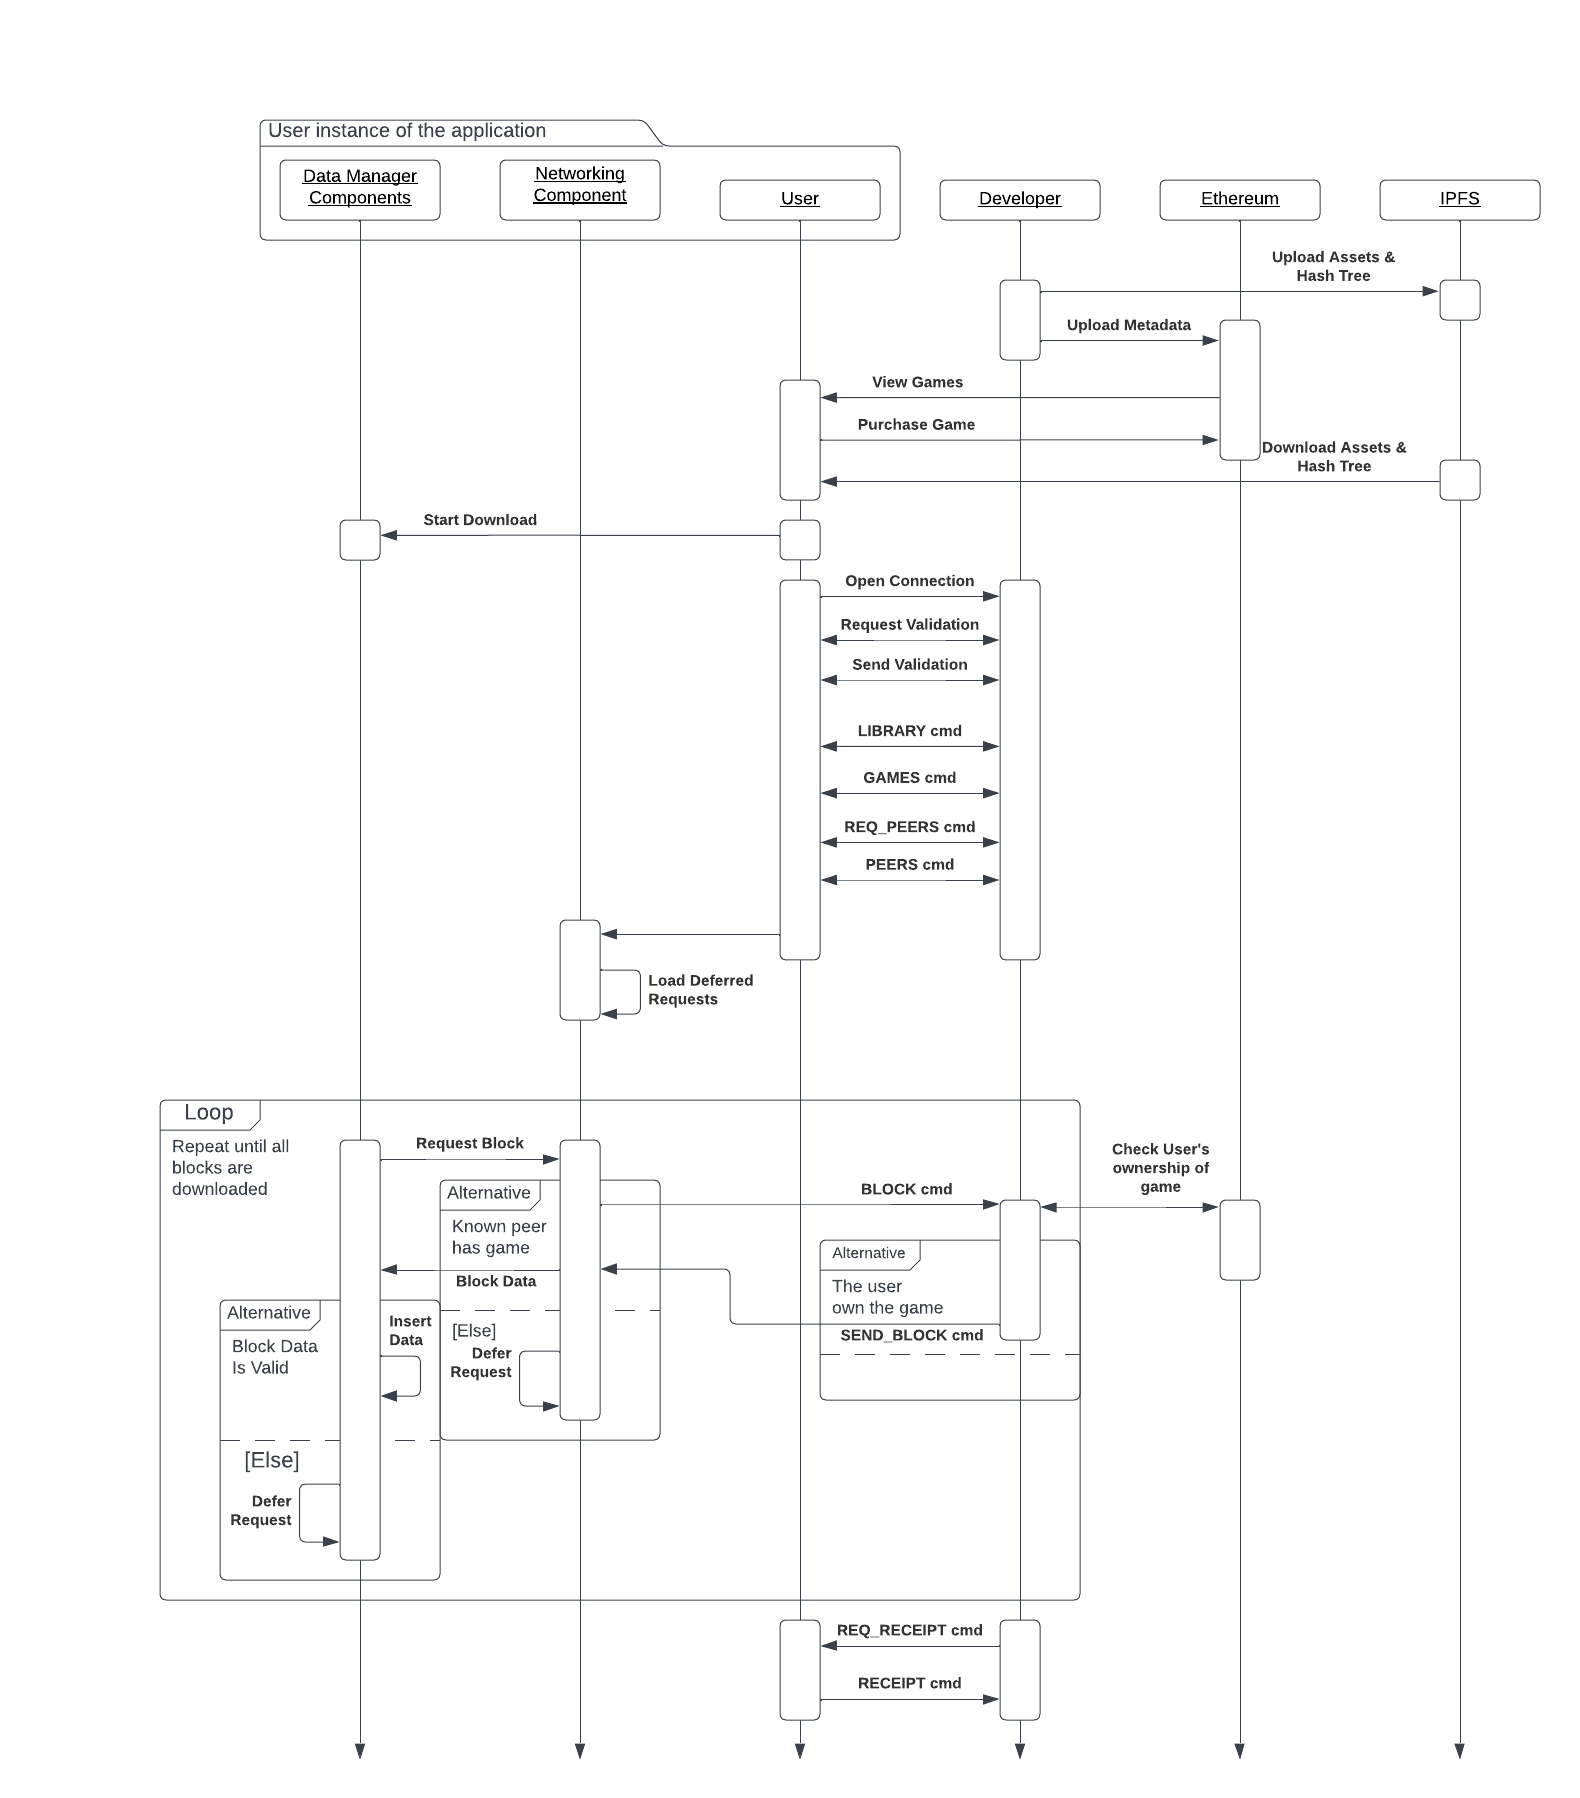
\includegraphics[width=\textwidth]{assets/images/diagrams/p2p-sequence.png}
  \caption{A sequence diagram showing the main interactions needed to download a game}
  \label{fig:p2p-interactions}
\end{figure}



\section{Benefits}\label{des:benefits}

This application presents the following benefits when compared with centralised game marketplaces:

\begin{itemize}
  \item \textbf{Privacy} A user's personal information and usage isn't collected. Traditional platforms require users to enter personal information and will actively collect data about a user's actions through the platform.
  \item \textbf{Ownership} A user's ownership of a game isn't tied to a single platform and use of Ethereum means that a user's ownership is upheld by all computers in the network.
  \item \textbf{Censorship} Similar to the previous point, no one party has control over the platform so it is much harder for third parties, such as governments, to restrict the content uploaded to it.
  \item \textbf{Profits} Developers and gamers communicate directly and this means developer's won't have to pay a hefty fee for a middle-man. This will result in potentially larger profits for the developers.  
\end{itemize}

\section{Limitations}\label{sec:design-lim}

This application presents the following limitations when compared with a centralised game marketplace:

\begin{itemize}
  \item \textbf{No Social Features} Social features, such as friends or achievements, were not included within the scope of this project.
  \item \textbf{Availability} Section~\ref{subsec:availability} highlights the issue of availability within P2P file-sharing systems and it is likely this platform will face similar issues.
  The use of a contribution system was implemented to help identify those users who have been contributing but there is no automatic rewards system\footnote{An example would be how the micro-payment system works in Swarm~\cite{hartman_swarm_1999}}.
  \item \textbf{Inefficient Updates} As updates are treated as individual games, they will require users to download the entire game again. This is highly inefficient and results in lots of duplicate data being downloaded.
  \item \textbf{Illegal Content} Currently there is no policy, automated or otherwise, to stop the distribution of illegal content. This is an incredibly complex problem to tackle and any obvious solution would risk violating the anti-censorship goal of this project. 
\end{itemize}

\newpage
\section{Sequence Diagram}

Figure~\ref{fig:p2p-interactions} shows how all of the components from this section are combined to download a game off of a single peer in the network.

\begin{figure}[H]
  \centering\hspace{-16.5mm}
  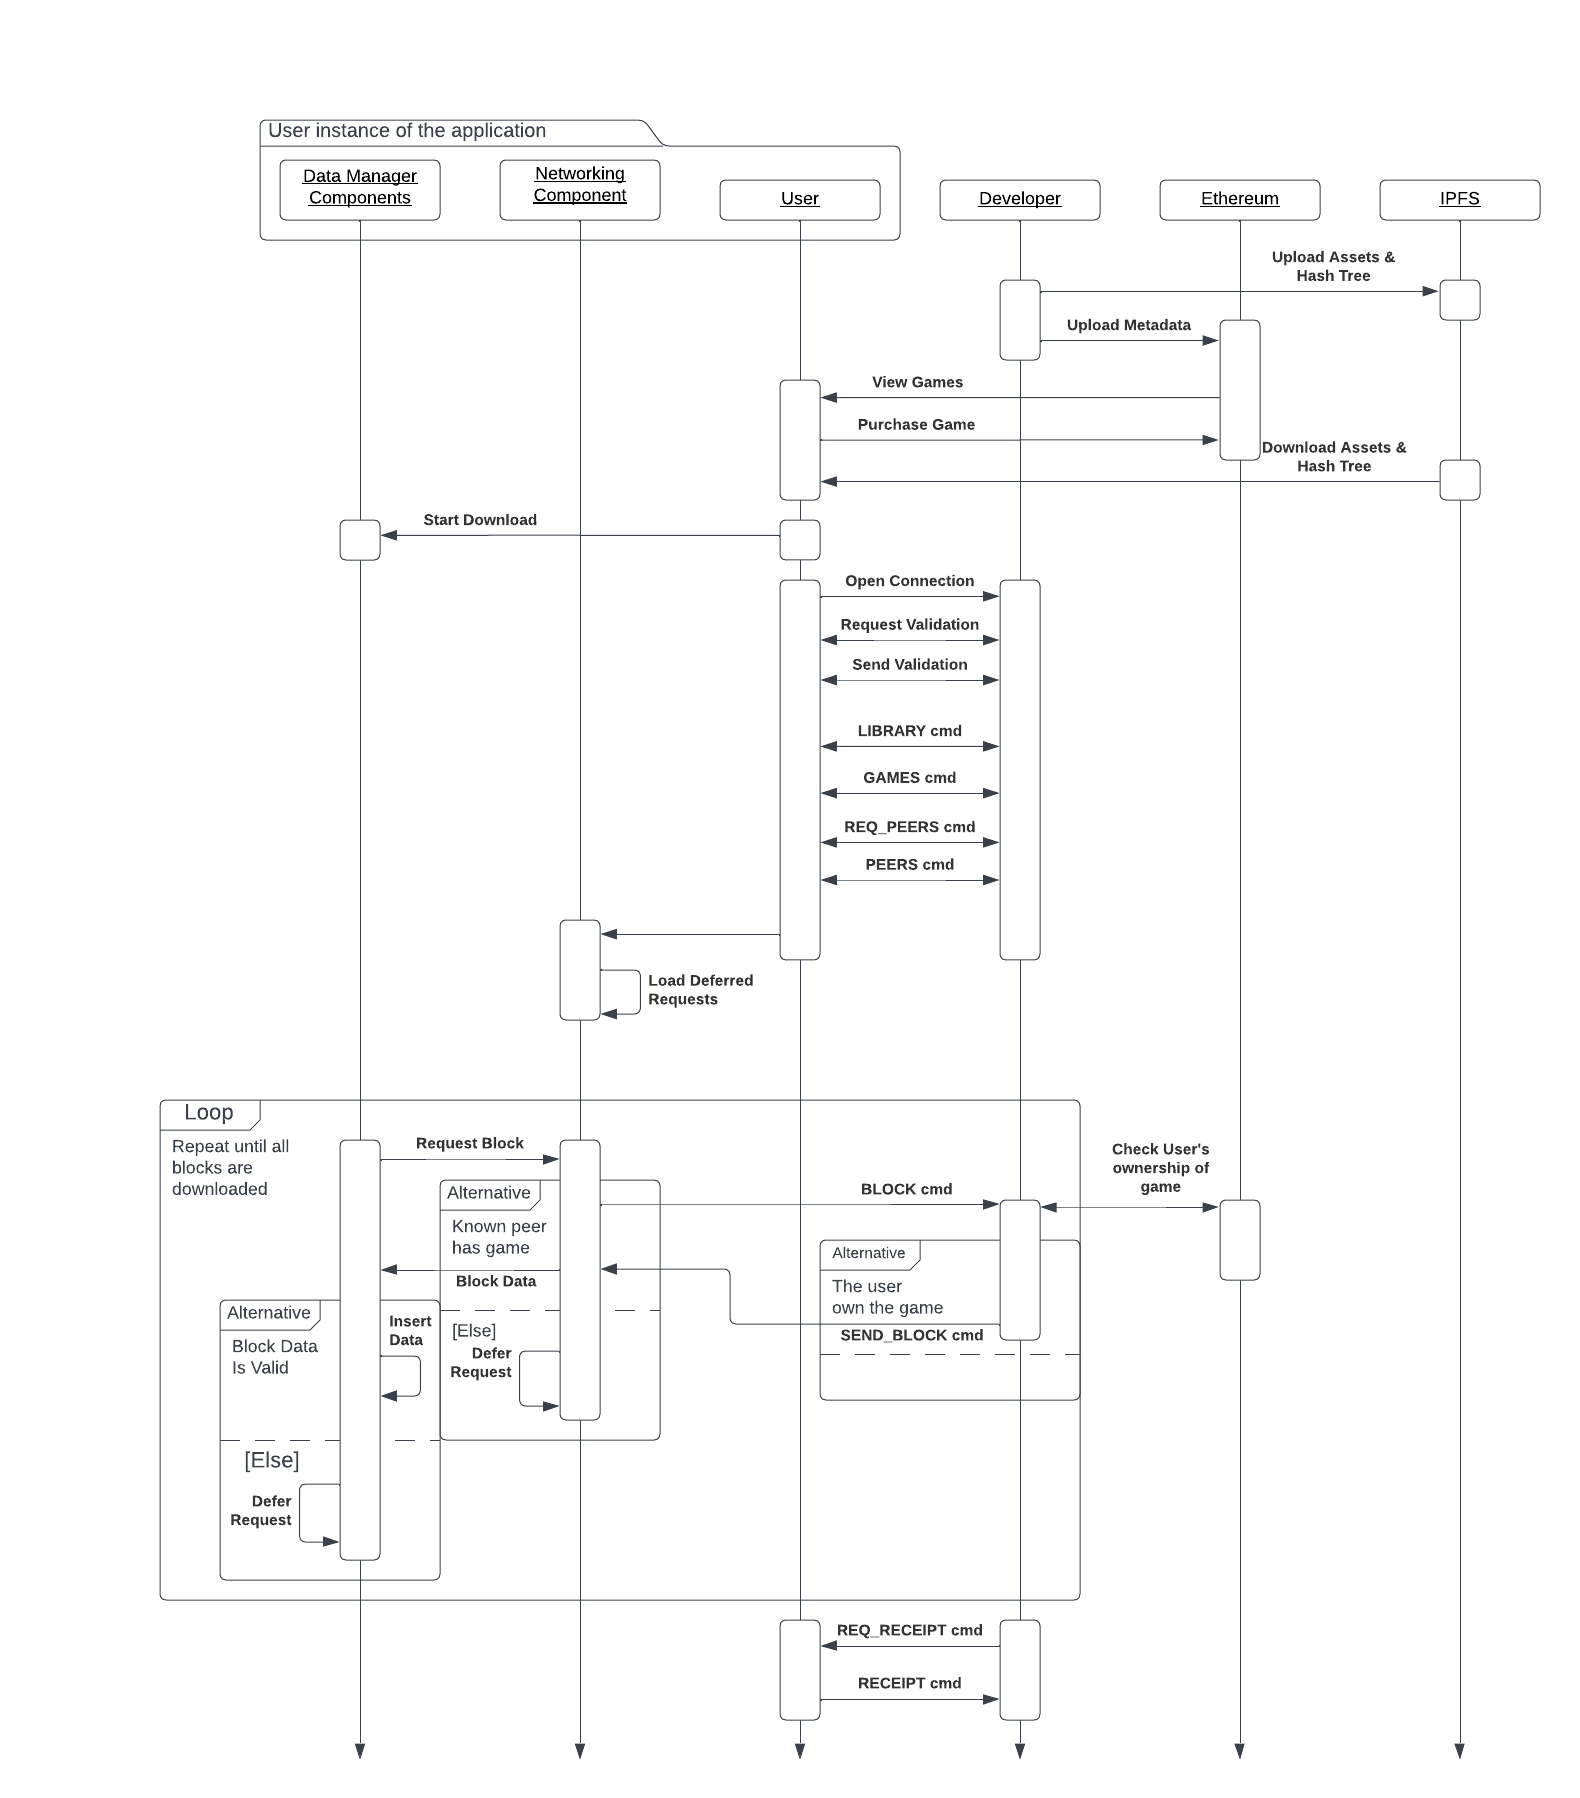
\includegraphics[width=1.1\textwidth]{assets/images/diagrams/p2p-sequence.png}
  \caption{A sequence diagram showing the main interactions needed to download a game from a single peer}
  \label{fig:p2p-interactions}
\end{figure}